% !TEX root = rCRF.tex
\section{Experimental Results}
In order to experimentally evaluate the proposed rCRF model and the belief computation, we perform experiments on two applications. Firstly, we estimate a belief over the activity a human is performing and the affordances of the objects in the scene by using the RGB-D video. After computing the belief, we detect the most likely activity and affordance sequences and study the improvement in the detection accuracy. Secondly, we test the accuracy of the beliefs in the anticipation setting. Indeed, we show that it is possible to obtain high-quality detection and anticipation via rCRF.

\begin{figure}[ht]
\small
%\begin{singlespace}
\begin{tabular}{p{5mm}@{}l}
\begin{tabular}{r}
\rotatebox[origin=r]{90}{\;\;\;\;\;\;\;Middle Frame}\\
\rotatebox[origin=l]{90}{Belief\;\;\;\;\;\;\;}
\end{tabular}
&
\begin{tabular}{p{3.7cm}p{3.7cm}p{3.7cm}p{3.7cm}}
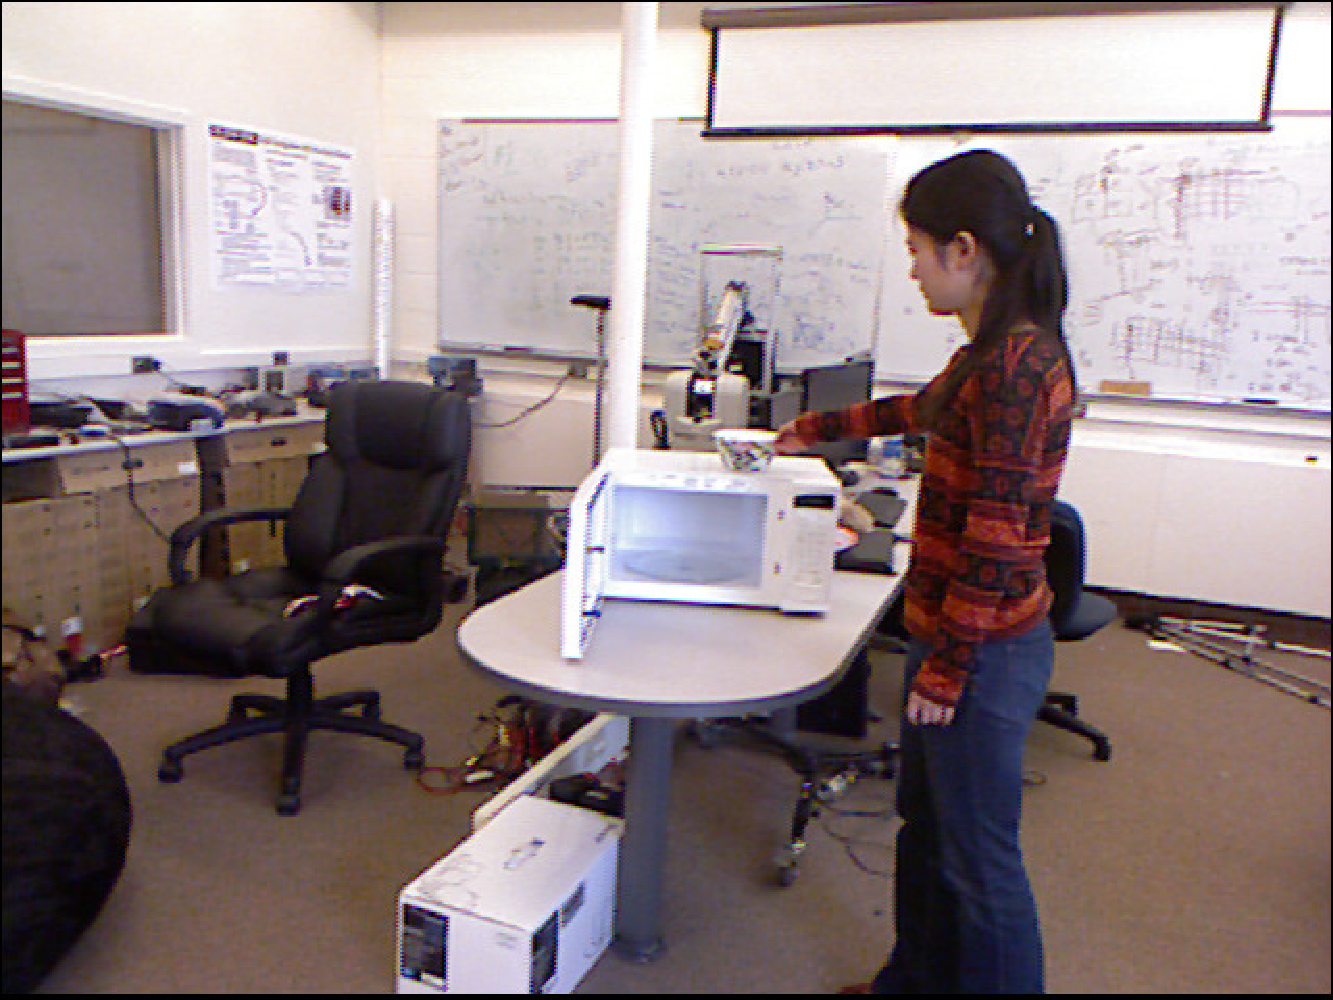
\includegraphics[width=0.225\textwidth]{f10} &
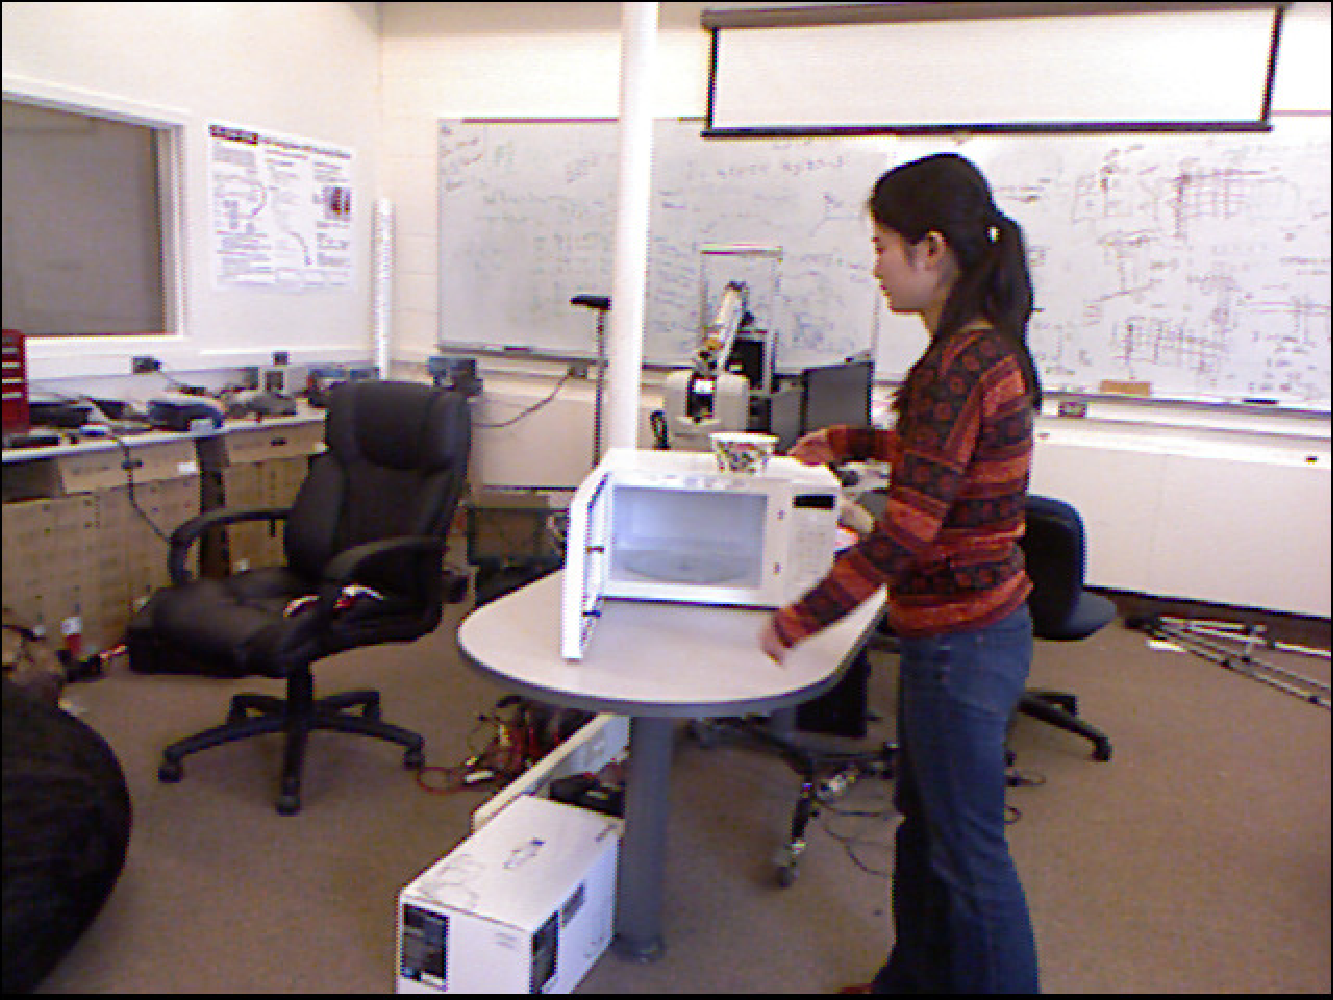
\includegraphics[width=0.225\textwidth]{f11} &
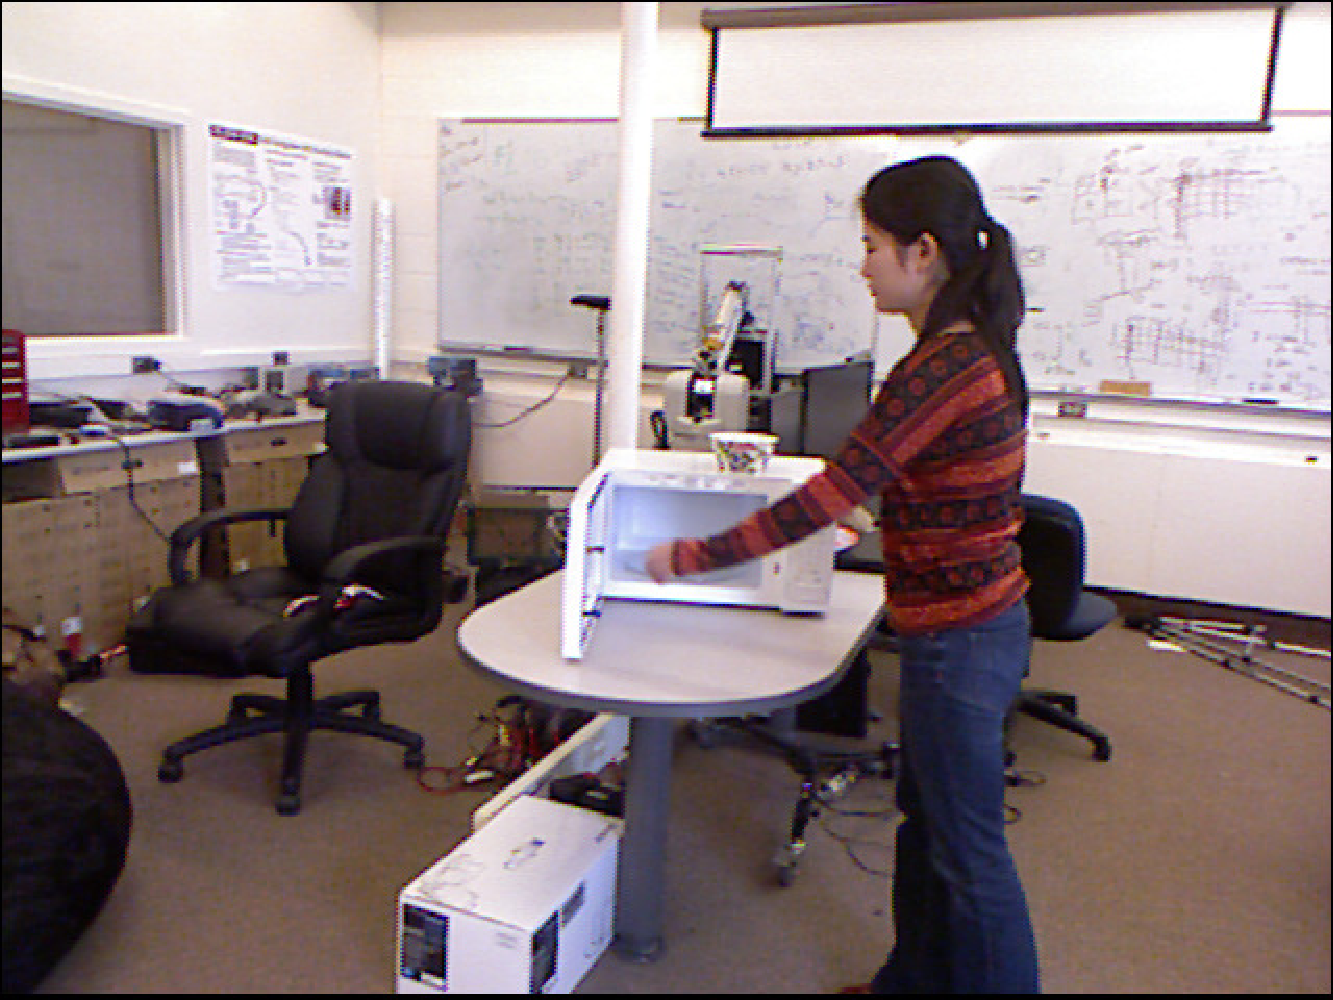
\includegraphics[width=0.225\textwidth]{f12} &
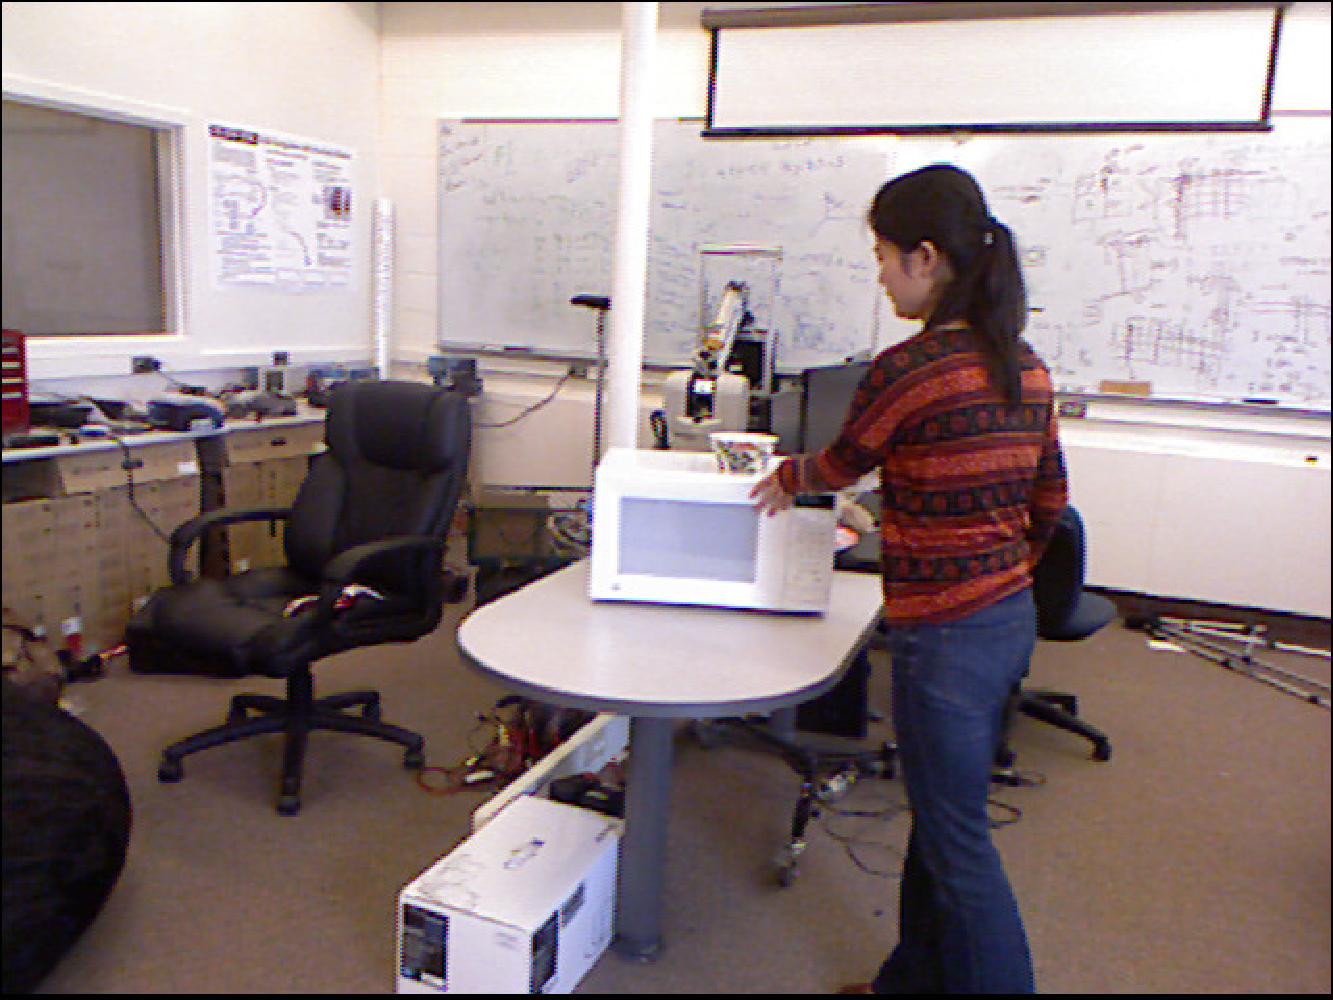
\includegraphics[width=0.225\textwidth]{f13}  \\ %\\%\begin{tabular}{p{3.6cm}p{3.6cm}p{3.6cm}p{3.6cm}}
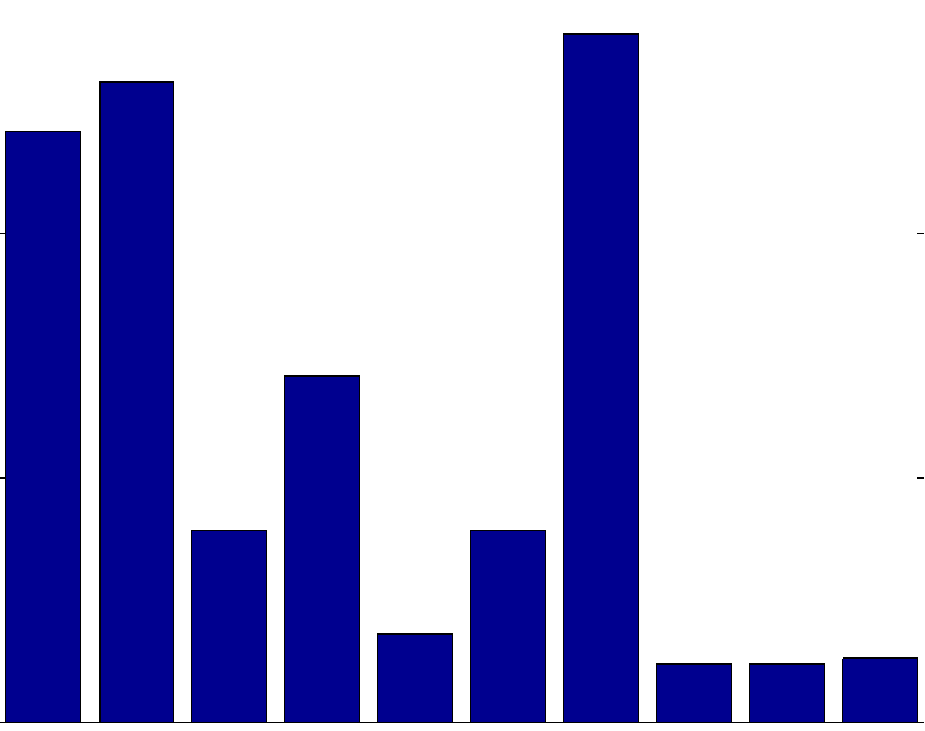
\includegraphics[width=0.225\textwidth, height=8mm]{P10} &
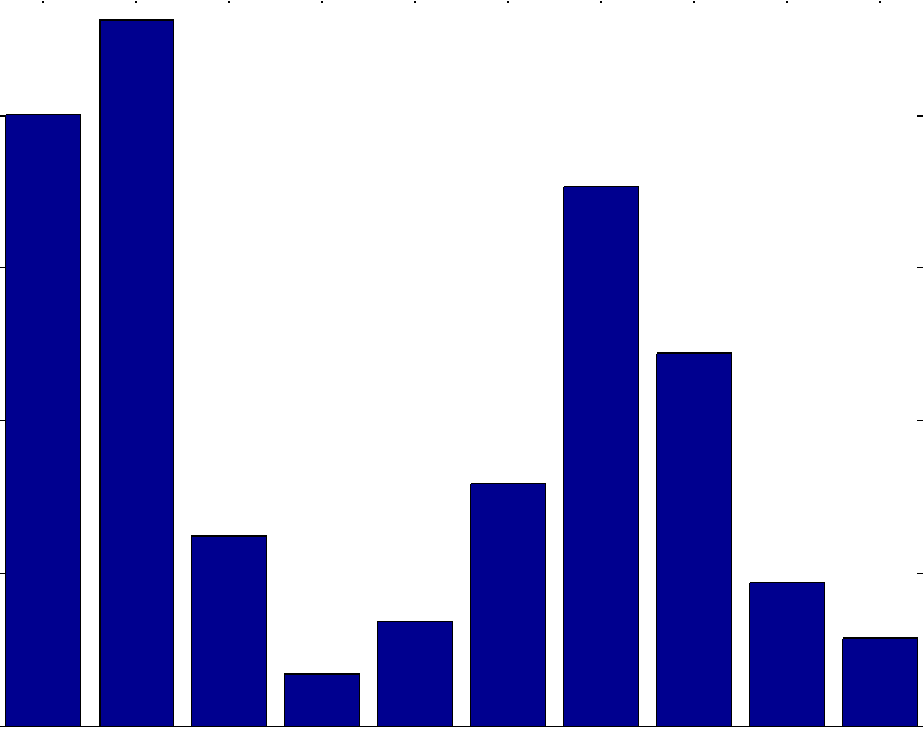
\includegraphics[width=0.225\textwidth, height=8mm]{P12P} &
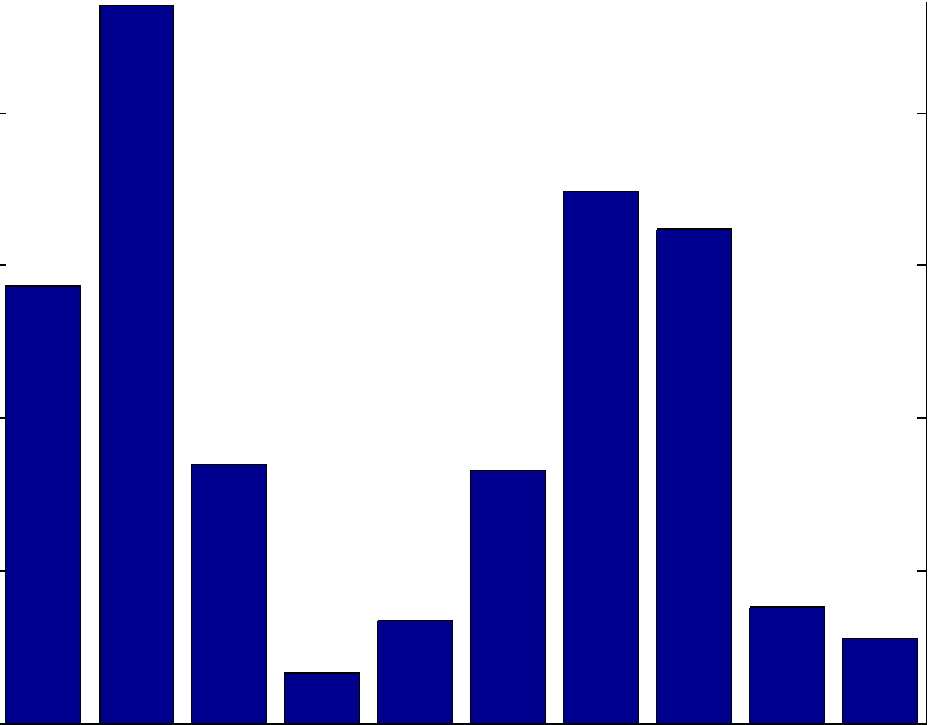
\includegraphics[width=0.225\textwidth, height=8mm]{P13P} &
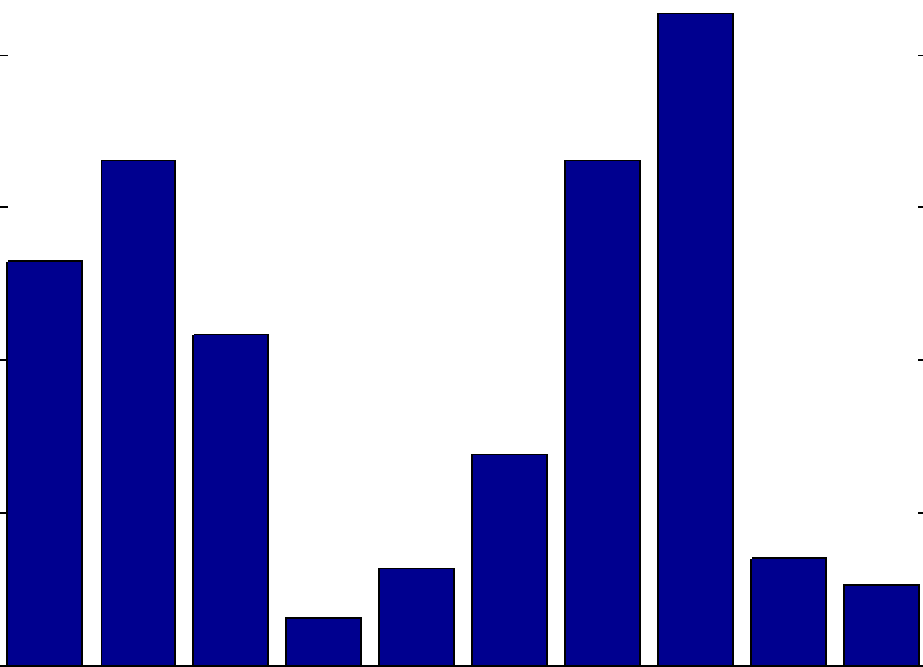
\includegraphics[width=0.225\textwidth, height=8mm]{P14P}  \\

\vspace{-6mm}\hspace{-1mm}\scalebox{0.84}{
\rotatebox[origin=r]{90}{reaching}\hspace{1mm}
\rotatebox[origin=r]{90}{moving}\hspace{1mm}
\rotatebox[origin=r]{90}{pouring}\hspace{1mm}
\rotatebox[origin=r]{90}{eating}\hspace{1mm}
\rotatebox[origin=r]{90}{drinking}\hspace{1mm}
\rotatebox[origin=r]{90}{opening}\hspace{1mm}
\rotatebox[origin=r]{90}{placing}\hspace{1mm}
\rotatebox[origin=r]{90}{closing}\hspace{1mm}
\rotatebox[origin=r]{90}{null}\hspace{1mm}
\rotatebox[origin=r]{90}{cleaning}}&
\vspace{-6mm}\hspace{-1mm}\scalebox{0.84}{
\rotatebox[origin=r]{90}{reaching}\hspace{1mm}
\rotatebox[origin=r]{90}{moving}\hspace{1mm}
\rotatebox[origin=r]{90}{pouring}\hspace{1mm}
\rotatebox[origin=r]{90}{eating}\hspace{1mm}
\rotatebox[origin=r]{90}{drinking}\hspace{1mm}
\rotatebox[origin=r]{90}{opening}\hspace{1mm}
\rotatebox[origin=r]{90}{placing}\hspace{1mm}
\rotatebox[origin=r]{90}{closing}\hspace{1mm}
\rotatebox[origin=r]{90}{null}\hspace{1mm}
\rotatebox[origin=r]{90}{cleaning}}&
\vspace{-6mm}\hspace{-1mm}\scalebox{0.84}{
\rotatebox[origin=r]{90}{reaching}\hspace{1mm}
\rotatebox[origin=r]{90}{moving}\hspace{1mm}
\rotatebox[origin=r]{90}{pouring}\hspace{1mm}
\rotatebox[origin=r]{90}{eating}\hspace{1mm}
\rotatebox[origin=r]{90}{drinking}\hspace{1mm}
\rotatebox[origin=r]{90}{opening}\hspace{1mm}
\rotatebox[origin=r]{90}{placing}\hspace{1mm}
\rotatebox[origin=r]{90}{closing}\hspace{1mm}
\rotatebox[origin=r]{90}{null}\hspace{1mm}
\rotatebox[origin=r]{90}{cleaning}}&
\vspace{-6mm}\hspace{-1mm}\scalebox{0.84}{
\rotatebox[origin=r]{90}{reaching}\hspace{1mm}
\rotatebox[origin=r]{90}{moving}\hspace{1mm}
\rotatebox[origin=r]{90}{pouring}\hspace{1mm}
\rotatebox[origin=r]{90}{eating}\hspace{1mm}
\rotatebox[origin=r]{90}{drinking}\hspace{1mm}
\rotatebox[origin=r]{90}{opening}\hspace{1mm}
\rotatebox[origin=r]{90}{placing}\hspace{1mm}
\rotatebox[origin=r]{90}{closing}\hspace{1mm}
\rotatebox[origin=r]{90}{null}\hspace{1mm}
\rotatebox[origin=r]{90}{cleaning}}
\end{tabular}
\end{tabular}

\begin{tabular}{p{5mm}@{}l}
\begin{tabular}{r}
\rotatebox[origin=r]{90}{\;\;\;\;\;\;\;Middle Frame}\\
\rotatebox[origin=l]{90}{Belief\;\;\;\;\;\;\;}
\end{tabular}
&
\begin{tabular}{p{3.7cm}p{3.7cm}p{3.7cm}p{3.7cm}}
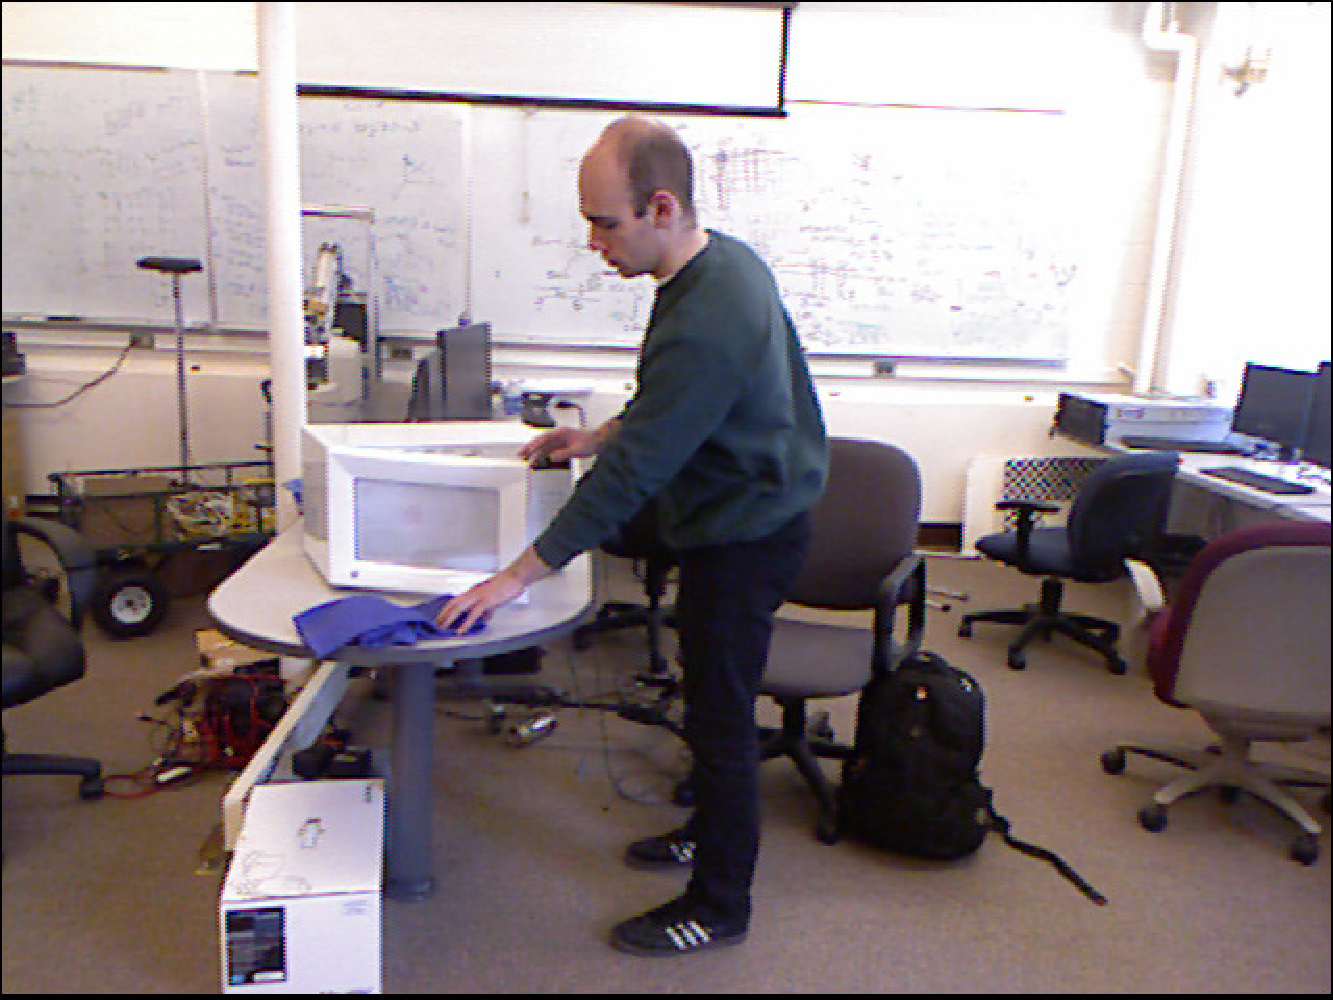
\includegraphics[width=0.225\textwidth]{l5} &
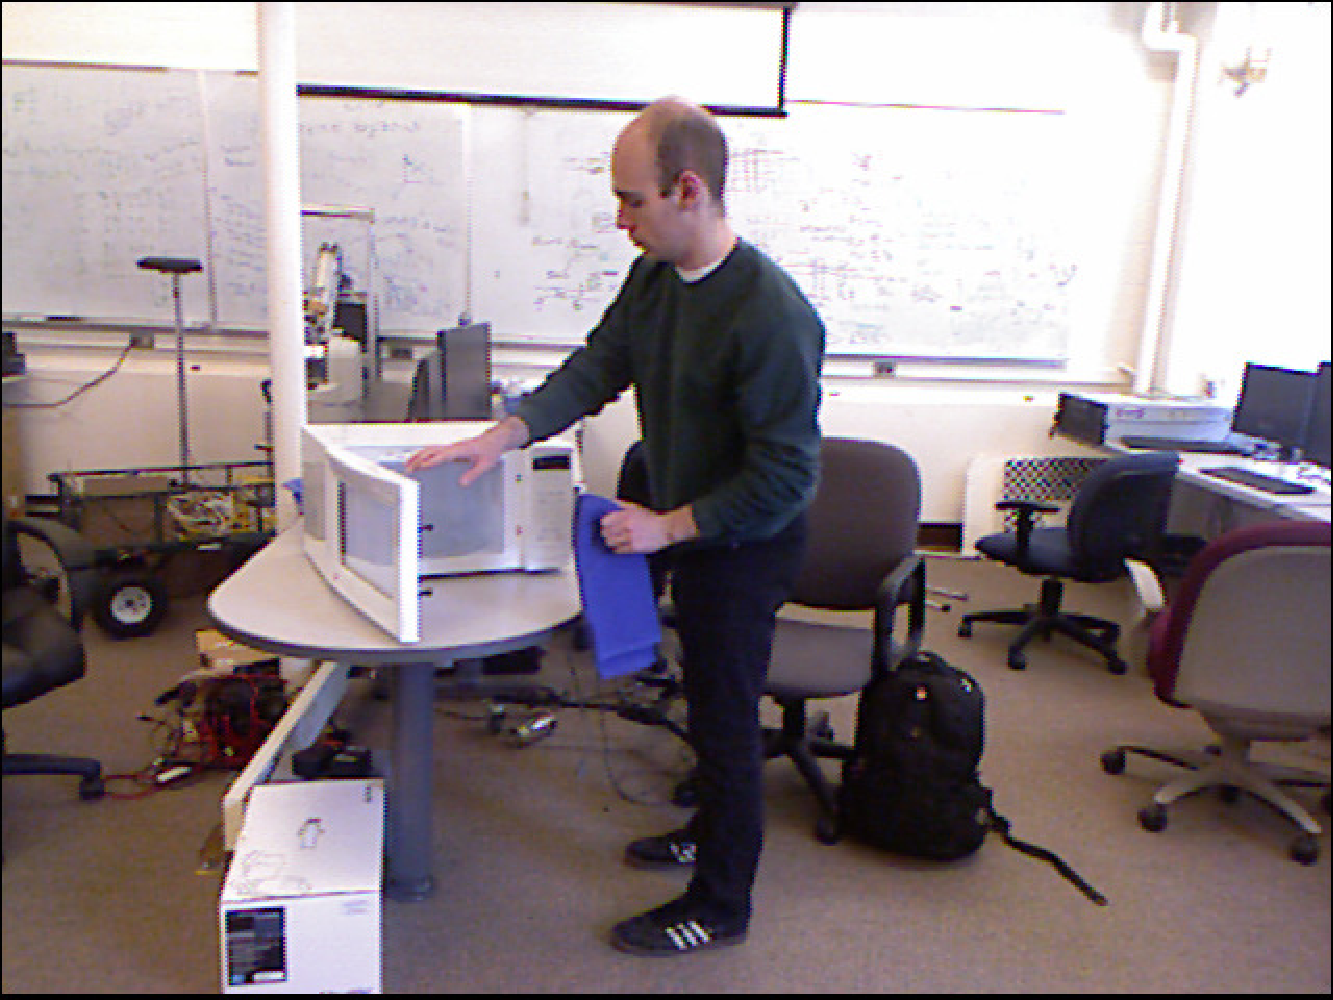
\includegraphics[width=0.225\textwidth]{l6} &
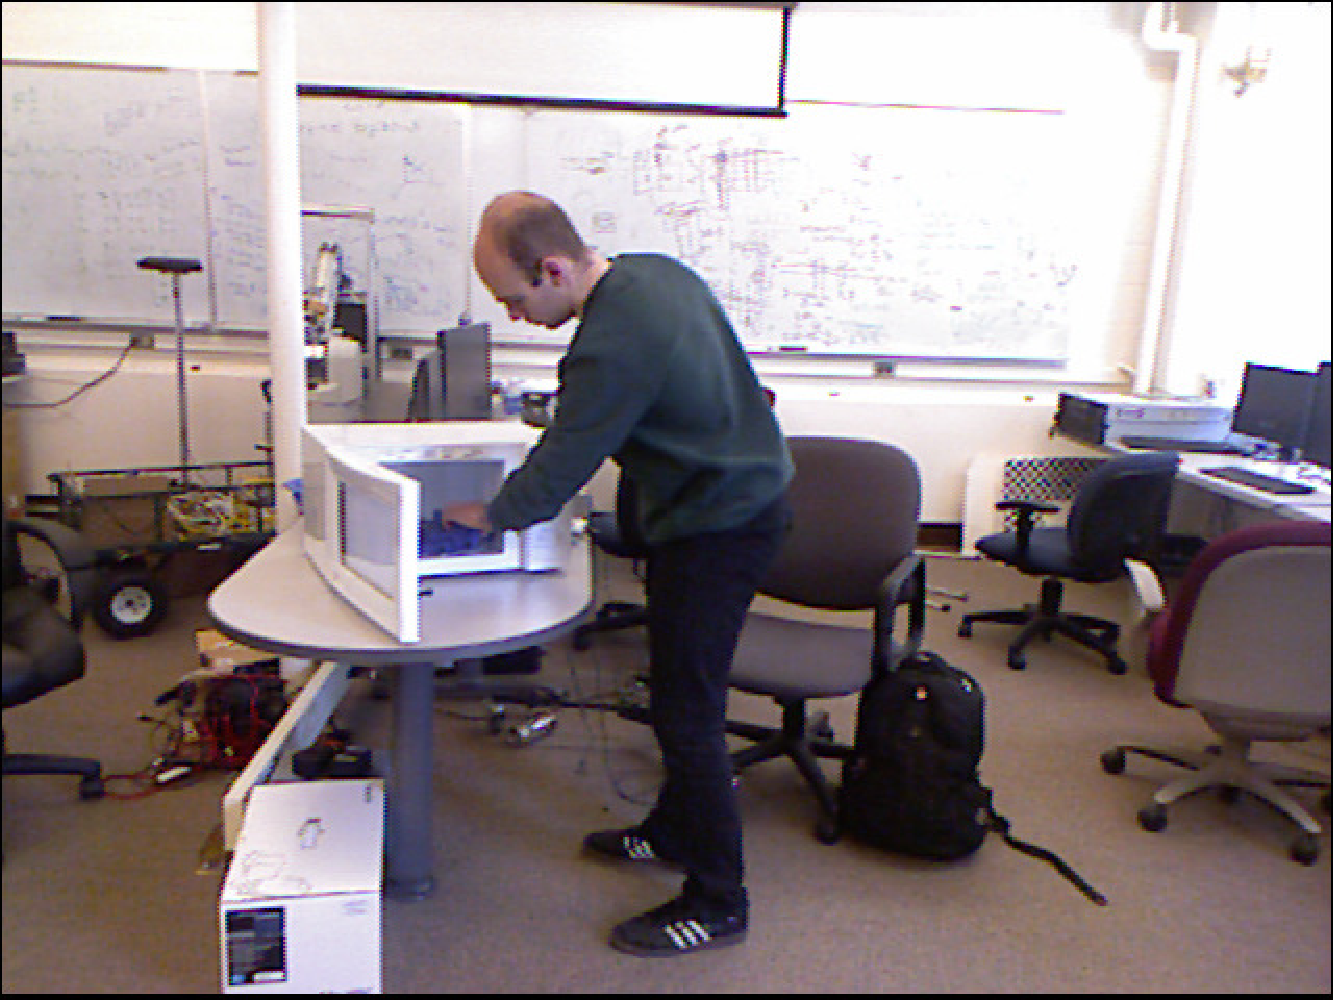
\includegraphics[width=0.225\textwidth]{l7} &
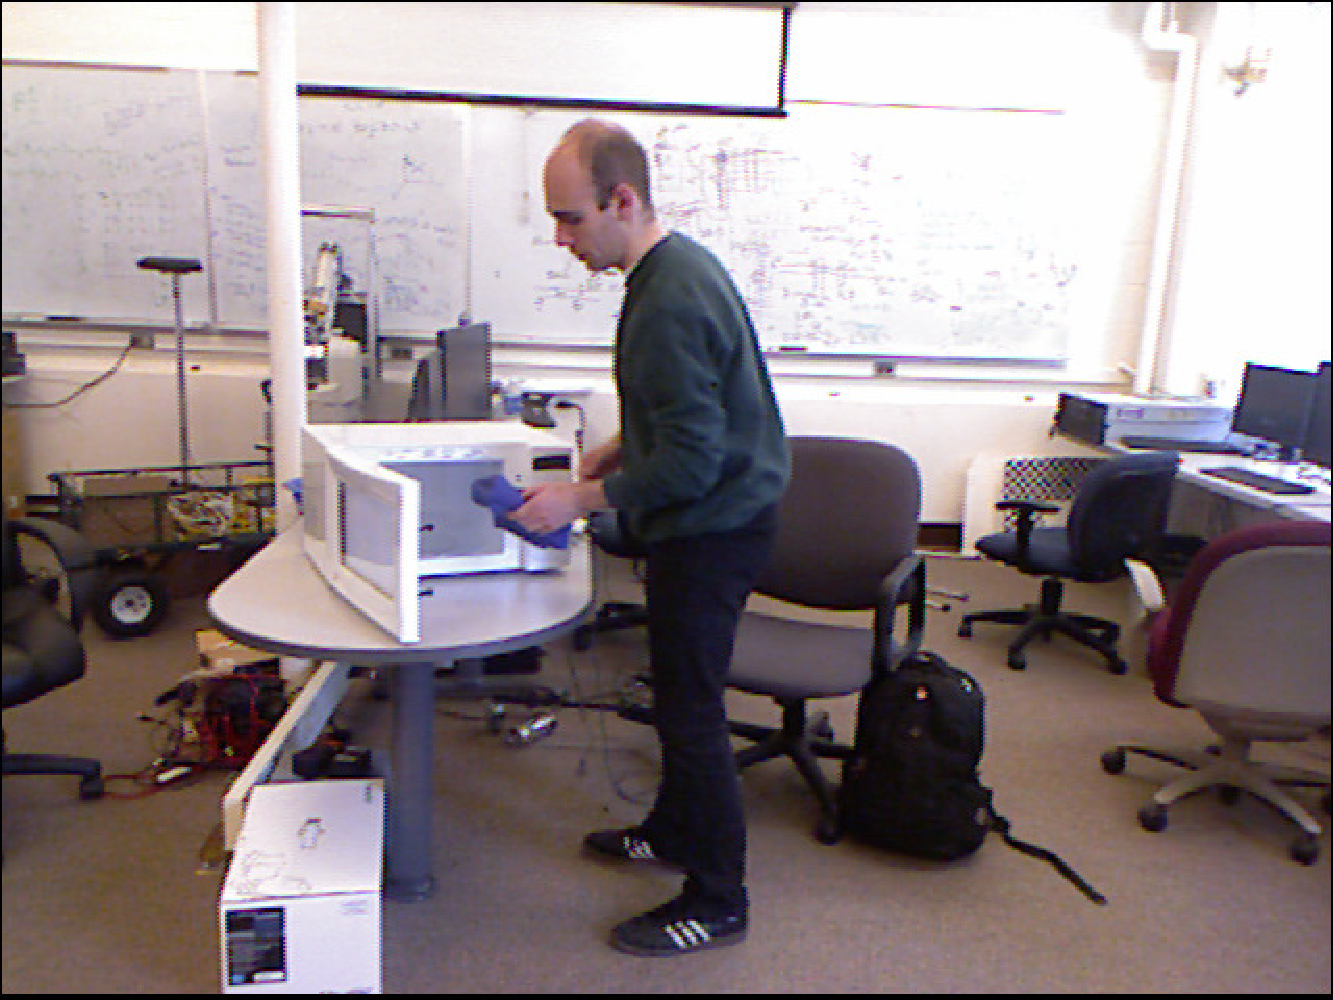
\includegraphics[width=0.225\textwidth]{l8}  \\
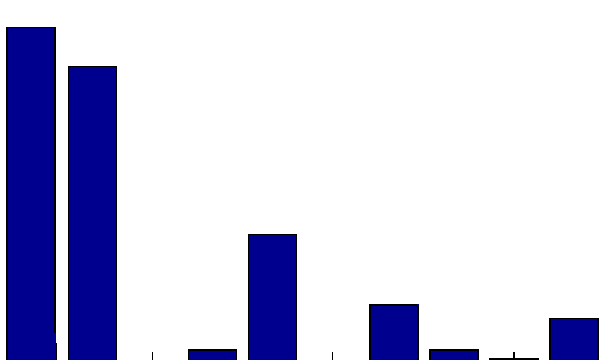
\includegraphics[width=0.225\textwidth, height=9mm]{bl5} &
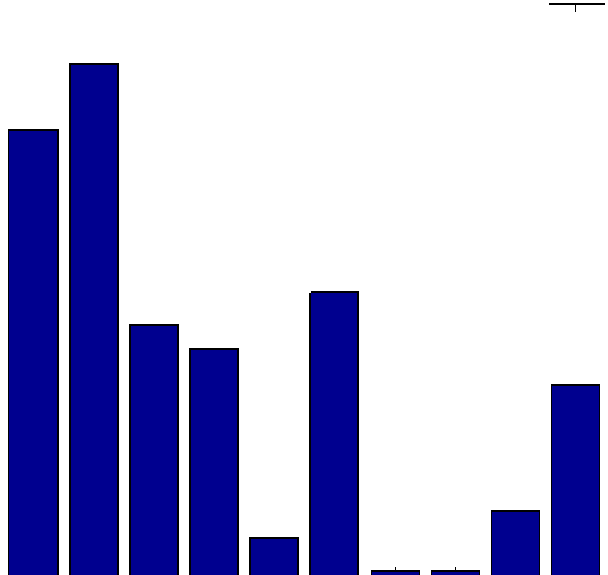
\includegraphics[width=0.225\textwidth, height=9mm]{bl6_2} &
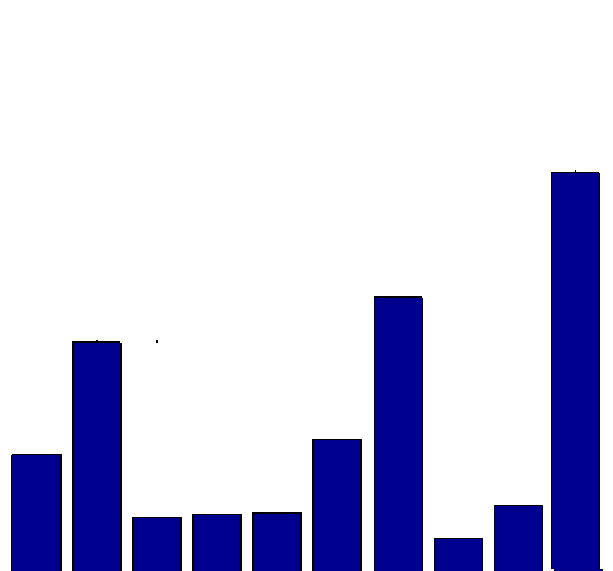
\includegraphics[width=0.225\textwidth, height=9mm]{bl7_2} &
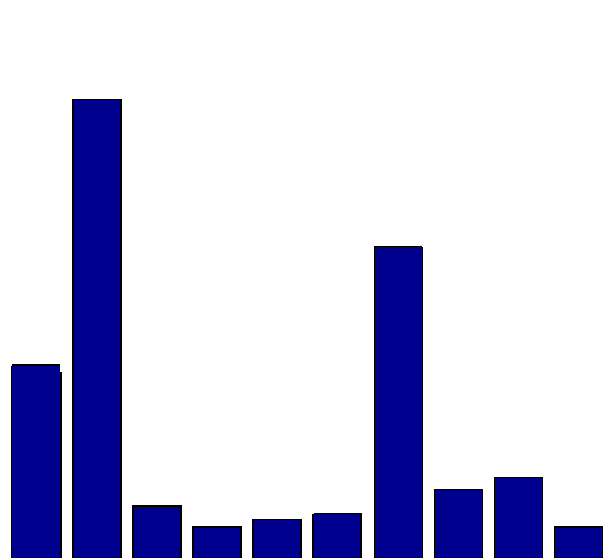
\includegraphics[width=0.225\textwidth, height=9mm]{bl8_2}  \\
\iffalse
\begin{tikzpicture}[remember picture,overlay]
\node[anchor=south west,inner sep=0] (image1)
  {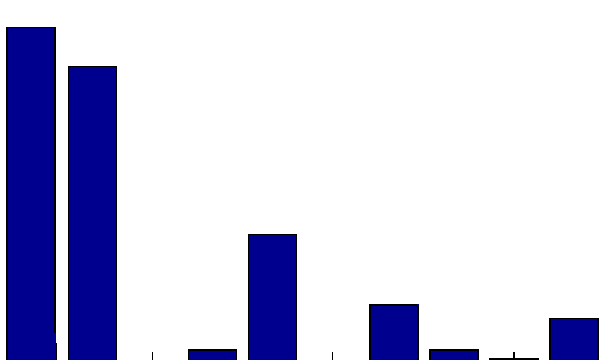
\includegraphics[width=0.22\textwidth, height=10mm]{bl5}};
\end{tikzpicture} &
\begin{tikzpicture}[remember picture,overlay]
\node[anchor=south west,inner sep=0] (image2)
  {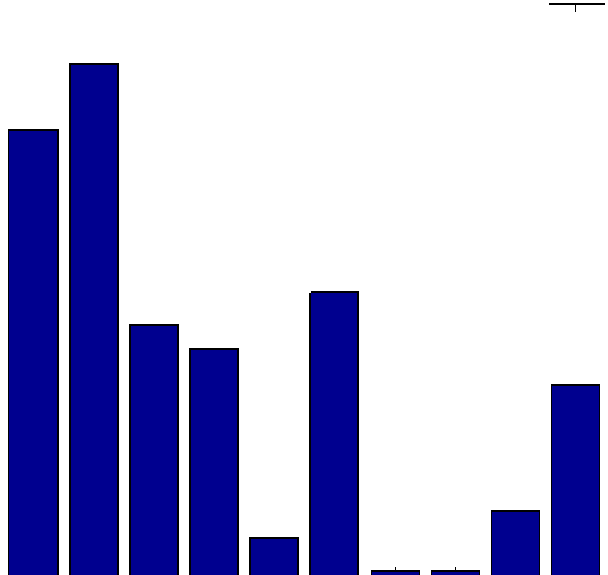
\includegraphics[width=0.22\textwidth, height=10mm]{bl6_2}};
\end{tikzpicture} &
\begin{tikzpicture}[remember picture,overlay]
\node[anchor=south west,inner sep=0] (image3)
  {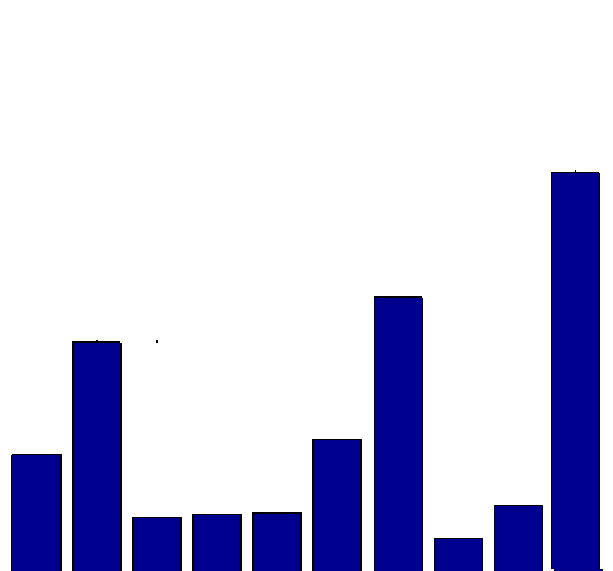
\includegraphics[width=0.22\textwidth, height=10mm]{bl7_2}};
\end{tikzpicture} &
\begin{tikzpicture}[remember picture,overlay]
\node[anchor=south west,inner sep=0] (image4)
  {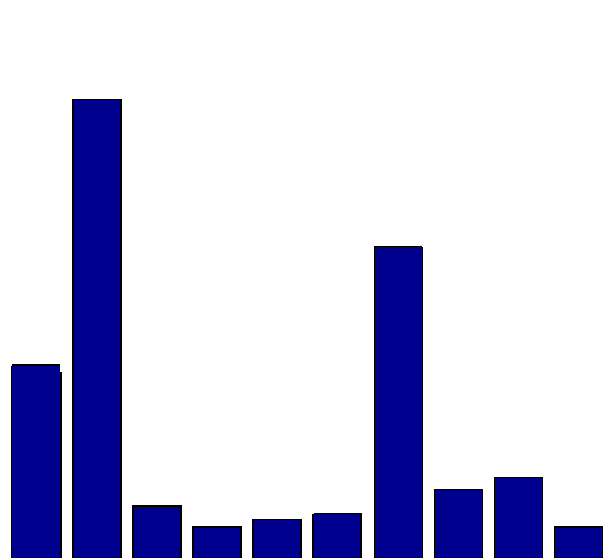
\includegraphics[width=0.22\textwidth, height=10mm]{bl8_2}};
\end{tikzpicture}
\begin{tikzpicture}[remember picture,overlay]
\draw[->,line width=2pt,red!80!black]
([yshift=-5pt,xshift=14pt]image4.west) |-
([yshift=-5pt,xshift=81pt]image3.west);
\draw[->,line width=2pt,red!80!black]
([yshift=0pt,xshift=81pt]image3.west) |-
([yshift=0pt,xshift=13pt]image2.west);
\draw[->,line width=2pt,red!80!black]
([yshift=-5pt,xshift=13pt]image2.west) |-
([yshift=-5pt,xshift=5pt]image1.west);
\end{tikzpicture}
\fi
\vspace{-6mm}\hspace{-1mm}\scalebox{0.84}{
\rotatebox[origin=r]{90}{reaching}\hspace{1mm}
\rotatebox[origin=r]{90}{moving}\hspace{1mm}
\rotatebox[origin=r]{90}{pouring}\hspace{1mm}
\rotatebox[origin=r]{90}{eating}\hspace{1mm}
\rotatebox[origin=r]{90}{drinking}\hspace{1mm}
\rotatebox[origin=r]{90}{opening}\hspace{1mm}
\rotatebox[origin=r]{90}{placing}\hspace{1mm}
\rotatebox[origin=r]{90}{closing}\hspace{1mm}
\rotatebox[origin=r]{90}{null}\hspace{1mm}
\rotatebox[origin=r]{90}{cleaning}}&
\vspace{-6mm}\hspace{-1mm}\scalebox{0.84}{
\rotatebox[origin=r]{90}{reaching}\hspace{1mm}
\rotatebox[origin=r]{90}{moving}\hspace{1mm}
\rotatebox[origin=r]{90}{pouring}\hspace{1mm}
\rotatebox[origin=r]{90}{eating}\hspace{1mm}
\rotatebox[origin=r]{90}{drinking}\hspace{1mm}
\rotatebox[origin=r]{90}{opening}\hspace{1mm}
\rotatebox[origin=r]{90}{placing}\hspace{1mm}
\rotatebox[origin=r]{90}{closing}\hspace{1mm}
\rotatebox[origin=r]{90}{null}\hspace{1mm}
\rotatebox[origin=r]{90}{cleaning}}&
\vspace{-6mm}\hspace{-1mm}\scalebox{0.84}{
\rotatebox[origin=r]{90}{reaching}\hspace{1mm}
\rotatebox[origin=r]{90}{moving}\hspace{1mm}
\rotatebox[origin=r]{90}{pouring}\hspace{1mm}
\rotatebox[origin=r]{90}{eating}\hspace{1mm}
\rotatebox[origin=r]{90}{drinking}\hspace{1mm}
\rotatebox[origin=r]{90}{opening}\hspace{1mm}
\rotatebox[origin=r]{90}{placing}\hspace{1mm}
\rotatebox[origin=r]{90}{closing}\hspace{1mm}
\rotatebox[origin=r]{90}{null}\hspace{1mm}
\rotatebox[origin=r]{90}{cleaning}}&
\vspace{-6mm}\hspace{-1mm}\scalebox{0.84}{
\rotatebox[origin=r]{90}{reaching}\hspace{1mm}
\rotatebox[origin=r]{90}{moving}\hspace{1mm}
\rotatebox[origin=r]{90}{pouring}\hspace{1mm}
\rotatebox[origin=r]{90}{eating}\hspace{1mm}
\rotatebox[origin=r]{90}{drinking}\hspace{1mm}
\rotatebox[origin=r]{90}{opening}\hspace{1mm}
\rotatebox[origin=r]{90}{placing}\hspace{1mm}
\rotatebox[origin=r]{90}{closing}\hspace{1mm}
\rotatebox[origin=r]{90}{null}\hspace{1mm}
\rotatebox[origin=r]{90}{cleaning}}
\end{tabular}
\end{tabular}
\caption{\textbf{Anticipated belief over activity.} In the first and third row, we show a middle frame of the temporal segment. In the second and fourth row, we show the anticipated belief we computed for the middle frame. Note that frames are not visible to the algorithm and only included for evaluation.}
%\vspace{-4mm}
\label{abcd}
%\end{singlespace}
\end{figure}


\noindent {\bf Data:} We use CAD-120 \cite{hemaIJRR} dataset in order to evaluate our method. CAD-120 dataset includes 120 RGB-D videos of four different subject performing activities \emph{reaching, moving, pouring, etc.} while interacting with objects having affordances \emph{reachable, movable, pourable, etc.}. There are 10 activity classes and 12 object affordance classes.

\noindent {\bf Experimental Setup:} For computing the features and learning the CRF parameters, we follow the approach and the code in \cite{hemaIJRR}. Following the convention in \cite{hemaIJRR}, we use 4-fold cross-validation by training over the data from 3 subjects and testing on the remaining subject. We then average the results over 4-folds. We implemented the rCRF as we explain in Algorithm~\ref{alg:recursive} with the following parameters obtainded via cross-validation; we sampled $M=15$ diverse samples and ran the recursive message updates with the number of iterations limit as $5$.

For the anticipation setting, In order to experiment the $\tau$ seconds into the future anticipation, we experiment over all feasible anticipation scenarios. In other words, we anticipated the time instant $t+\tau$ by using the segments $1\ldots t$ for all $t<T-\tau$, where $T$ is the length of the video. Then, we averaged the score over all feasible experiments.

\noindent {\bf Baseline Algorithms:} In detection setting, we compare the detection results of the rCRF to MAP solution of the spatiotemporal CRF in \cite{hemaIJRR}. We also included the state-of-the art activity detection results from Hu et al. \cite{latentIcra}. Moreover, \cite{latentIcra} is not based on object affordances and it only outputs activity detections. For the anticipation, we compare the rCRF with the state-of-the-art anticipation methods ATCRF \cite{hemaAnt} and GP-LCRF\cite{gpcrf}. We also include DCRF\cite{ddcrf}. In order to evaluate the contribution of the recursive modeling and the structured diversity separately, we also compare the rCRF with a recursive approach without diversity and a diversity-based approach without recursive modeling baselines.

The DivMBest algorithm in \cite{divmbest} uses the diverse sampling method to sample CRFs defined over each frame separately. DivMBest\cite{divmbest} then finds the most likely sequence via Viterbi algorithm. Since it is missing the recursive modeling, it serves as \emph{structured diversity without recursive filtering} baseline. We replace the diversity-based sampling in our method with Gibbs sampler and consider it as \emph{recursive filtering approach without structured diversity} baseline. For the Gibbs sampling, we sampled $50$ samples per temporal segment. We denote the recursive approach with Gibbs sampling as \emph{\mbox{"rCRF w/o div"}} while tabulating the results.

\noindent {\bf Evaluation Metrics:} For activity detection, we compute the ratio of the correctly classified labels (\emph{micro precision}) and the averages of the precision and recall values computed for each activity and object affordance classes (\emph{macro precision} and \emph{macro recall}). For anticipation, we record the ratio of the correctly classified labels \emph{micro precision}, the average of the f-1 score that is computed for each activity and object affordance class (\emph{macro f-1 score}), and the precision of the top 3 anticipated labels (\emph{robot anticipation metric}). While computing the \emph{robot anticipation metric}; if any of the top 3 anticipation is correct, it is counted as true positive.

\noindent {\bf Accuracy of the rCRF in detection setting.}
We evaluate the rCRF for activity detection and summarize the results in Table~\ref{Tdet}. Table~\ref{Tdet} suggests that the rCRF outperforms the MAP solution \cite{hemaIJRR} and performs similarly with the state-of-the-art solution \cite{latentIcra}. Since rCRF and \cite{hemaIJRR} are using the same spatial relations, the performance difference is due to the modeling of the temporal relations in rCRF. We use \mbox{first-order} statistics as temporal dynamics, and they are quite accurate as shown in the heatmap in Figure~\ref{heatmap}. They also capture semantic information like objects become stationary after being used.

\begin{figure}
  \subfigure[Human Activity]{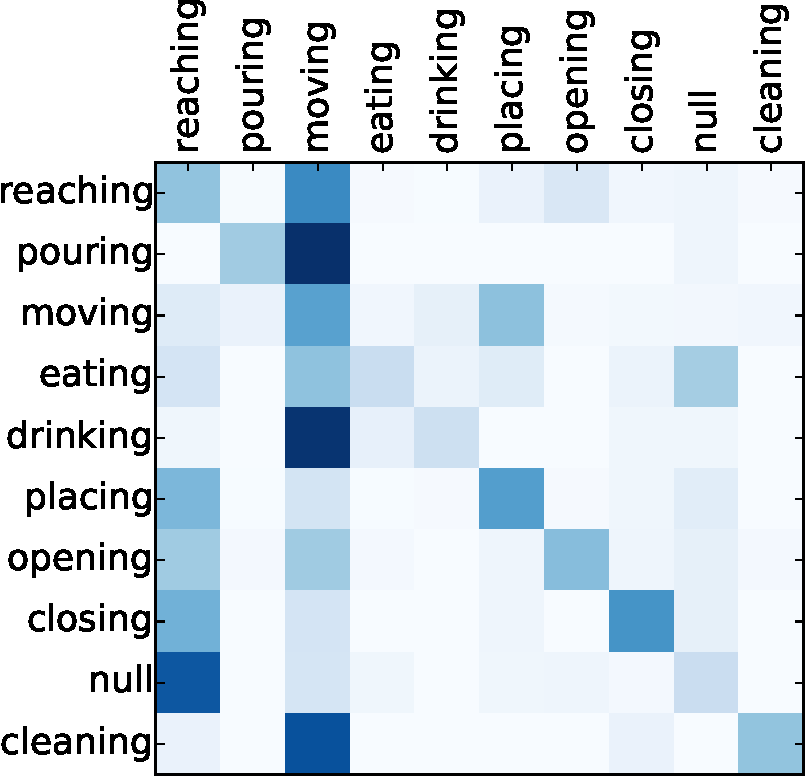
\includegraphics[width=0.48\textwidth]{tranAct}}~
  \subfigure[Object Affordance]{ 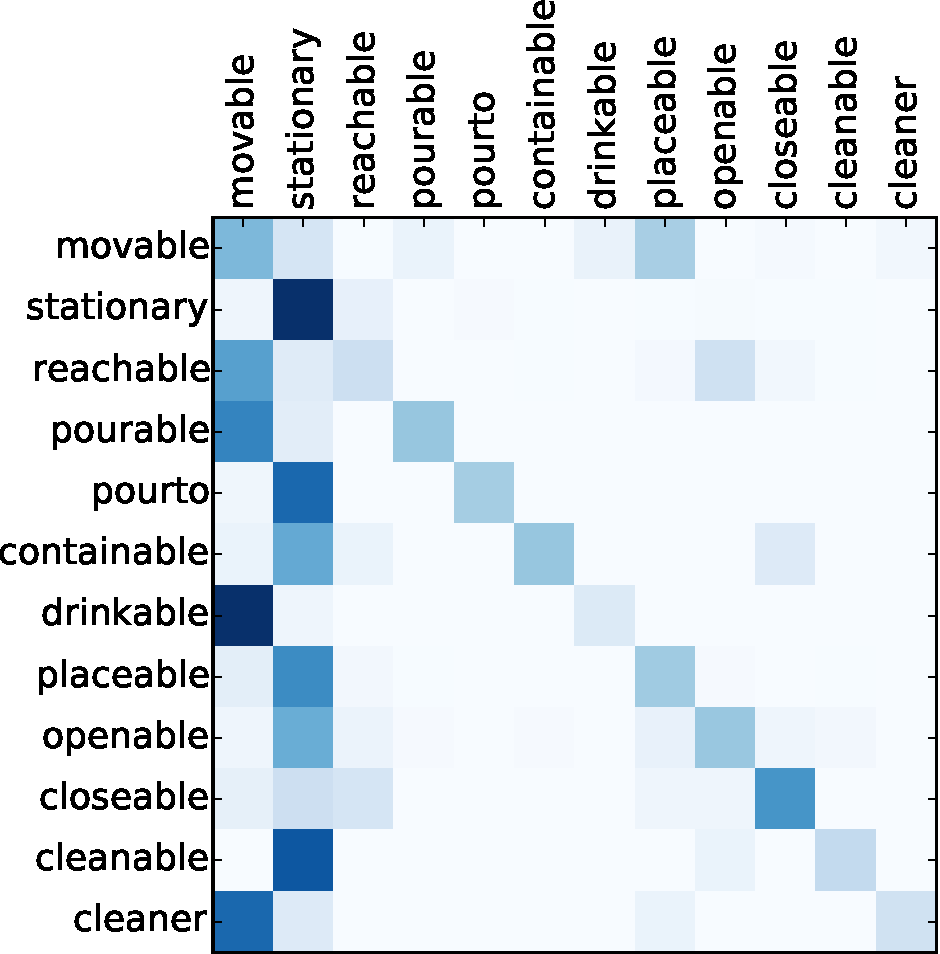
\includegraphics[width=0.48\textwidth]{tranObj}}
  \caption{Heatmap of the first-order statistics of activity and object affordance classes. They are used as temporal dynamics by rCRF.}
  \label{heatmap}
\end{figure}

\noindent {\bf Accuracy of the rCRF in anticipation setting.}
We evaluate the accuracy of the belief we compute via rCRF, both quantitatively and qualitatively. For qualitative evaluation, we show the segment that we are anticipating the belief over, as well as the belief we obtain in Figure~\ref{abcd}. Please note that, this visual information is not visible to the algorithm, and it is only included for the subjective evaluation.

As shown in the figure, anticipated belief is capturing the scene accurately. Belief is accurate even for the case of concurrent activities. For example, in the second column of the second row in Figure \ref{abcd}, subject is reaching the microwave and moving the cleaner. Our method assigns similar likelihood values to both reaching and moving.

We also perform quantitative analysis over anticipation accuracy. We anticipate 3 seconds into the future and summarize the results in Table~\ref{Tant}. As shown in the Table~\ref{Tant}, rCRF outperforms the state-of-the-art heuristic method \cite{hemaAnt} and the GP-LCRF method \cite{gpcrf} significantly as well as all other baselines. We believe this result is due to the accurate joint-modeling of the temporal relations and the CRF model. We further analysed this behaviour in the subsequent sections.

\begin{table}[ht]
\centering
\tabcolsep=0.7mm
\footnotesize
%\vspace{-1mm}
\caption{\textbf{Detection Performance over CAD-120.}  We compare rCRF with MAP solution and baselines for detections accuracy.}
%\vspace{-1mm}
\begin{tabular}{@{}l@{}|ccc|ccc@{}} \hline
& \multicolumn{3}{@{}|c@{}}{Sub-activity } &   \multicolumn{3}{@{}|c@{}}{Object Affordance } \\ \hline
& micro & \multicolumn{2}{@{}c|@{}}{macro} &   micro & \multicolumn{2}{@{}c@{}}{macro} \\
% \hline
 & prec(\%) & prec(\%) & rec(\%) &   prec(\%) & prec(\%) & rec(\%) \\
\hline
Chance & $10.0${\scriptsize $\pm 0.1$}  & $10.0${\scriptsize $\pm 0.1$}  & $10.0${\scriptsize $\pm 0.1$}  & $8.3${\scriptsize $\pm 0.1$}  & $8.3${\scriptsize $\pm 0.1$}  & $8.3${\scriptsize $\pm 0.1$}  \\
Hu et al.\cite{latentIcra} & $67.8${\scriptsize $\pm 1.4$}  &  $65.5${\scriptsize $\pm 3.5$}&  $\mathbf{63.5}${\scriptsize $\mathbf{\pm 6.6}$}  & N/A & N/A & N/A \\
MAP Sol\cite{hemaIJRR} & $63.4${\scriptsize $\pm 1.6$}  &  $65.3${\scriptsize $\pm 2.3$}&  $54.0${\scriptsize $\pm 4.6$}  & $79.4${\scriptsize $\pm 0.8$} & $62.5${\scriptsize $\pm 5.4$} & $50.2${\scriptsize $\pm 4.9$} \\
DivMBest\cite{divmbest}& $64.0${\scriptsize $\pm 1.3$} & $61.7${\scriptsize $\pm 2.1$} & $56.4${\scriptsize $\pm 2.7$} & $80.1${\scriptsize $\pm 1.0$} & $76.2${\scriptsize $\pm 2.5$} & $53.2${\scriptsize $\pm 3.2$} \\
DCRF\cite{ddcrf}& $61.2${\scriptsize $\pm 2.1$} & $62.8${\scriptsize $\pm 2.8$} & $54.3${\scriptsize $\pm 1.5$} & $71.9${\scriptsize $\pm 2.9$} & $80.6${\scriptsize $\pm 2.4$} & $62.5${\scriptsize $\pm 3.6$} \\
rCRF w/o div& $61.2${\scriptsize $\pm 1.8$} & $64.0${\scriptsize $\pm 1.8$} & $52.7${\scriptsize $\pm 3.8$} & $75.2${\scriptsize $\pm 2.4$} & $79.3${\scriptsize $\pm 3.1$} & $63.7${\scriptsize $\pm 2.9$} \\
rCRF&  $\mathbf{68.1}${\scriptsize$\mathbf{\pm 1.3}$} & $\mathbf{66.1}${\scriptsize $\mathbf{\pm 2.7}$} & $57.2${\scriptsize $\pm 3.9$} & $\mathbf{81.5}${\scriptsize $\mathbf{\pm 1.1}$} & $\mathbf{85.2}${\scriptsize $\mathbf{\pm 2.4}$} & $\mathbf{71.6}${\scriptsize $\mathbf{\pm 3.9}$} \\
\hline
\end{tabular}
%\end{singlespace}
\label{Tdet}
\end{table}
\begin{table}[ht]
\centering
\tabcolsep=0.7mm
\footnotesize
\vspace{-1mm}
\caption{\textbf{Anticipation performance for the anticipating 3 seconds in the future.} We compare rCRF with state-of-the-art anticipation algorithm and baselines for anticipation accuracy.}
\vspace{-1mm}
\begin{tabular}{@{}l@{}|ccc|ccc@{}} \hline
& \multicolumn{3}{@{}|c@{}}{Sub-activity } &   \multicolumn{3}{@{}|c@{}}{Object Affordance } \\ \hline
& micro & macro & robot ant. &  micro & macro & robot ant.   \\
Method & prec(\%) & f1-scr(\%) & metric(\%) & prec(\%) & f1-scr(\%) & metric(\%) \\ \hline
Chance & $10.0${\scriptsize $\pm 0.1$} & $10.0${\scriptsize $\pm 0.1$}  & $30.0${\scriptsize $\pm 0.1$} & $8.3${\scriptsize $\pm 0.1$} & $8.3${\scriptsize $\pm 0.1$}  & $24.9${\scriptsize $\pm 0.1$}  \\
GP-LCRF \cite{gpcrf} & $52.1${\scriptsize $\pm 1.2$} & $43.2${\scriptsize $\pm 1.5$} &  $76.1${\scriptsize $\pm 1.5$}  & $68.1${\scriptsize$\pm 1.0$}  & $44.2${\scriptsize $\pm 1.2$}  & $74.9${\scriptsize $\pm 1.1$}  \\
ATCRF \cite{hemaAnt} & $47.7${\scriptsize $\pm 1.6$} & $37.9${\scriptsize $\pm 2.6$} &  $69.2${\scriptsize $\pm 2.1$}  & $66.1${\scriptsize $\pm 1.9$}  & $36.7 ${\scriptsize $\pm 2.3$}  & $71.3${\scriptsize $\pm 1.7$}  \\
DivMBest\cite{divmbest}& $47.9${\scriptsize $\pm 1.4$} & $43.2${\scriptsize $\pm 3.6$} & $71.5${\scriptsize $\pm 2.7$} & $61.3${\scriptsize $\pm 1.4$} & $56.3 ${\scriptsize $\pm 2.1$} & $73.3${\scriptsize $\pm 0.5$} \\
DCRF\cite{ddcrf}& $48.3${\scriptsize $\pm 2.6$} & $35.4${\scriptsize $\pm 1.8$} & $66.6${\scriptsize $\pm 1.1$} &
$55.2${\scriptsize $\pm 3.1$} & $48.5${\scriptsize $\pm 3.1$} & $71.24${\scriptsize $\pm 2.2$} \\
rCRF w/o div& $49.6${\scriptsize $\pm 2.1$} & $39.7${\scriptsize $\pm 2.6$} & $65.1${\scriptsize $\pm 1.1$} & $56.2${\scriptsize $\pm 1.9$} & $47.4${\scriptsize $\pm 3.1$} & $70.8${\scriptsize $\pm 2.5$} \\
rCRF & $\mathbf{54.3}${\scriptsize $\mathbf{\pm 3.9}$} & $\mathbf{45.8}${\scriptsize $\mathbf{\pm 2.7}$} & $\mathbf{76.5}${\scriptsize $\mathbf{\pm 2.6 }$}  & $\mathbf{78.7}${\scriptsize $\mathbf{\pm 3.4}$} &$\mathbf{74.9}${\scriptsize $\mathbf{\pm 3.8}$} & $\mathbf{82.1}${\scriptsize $\mathbf{\pm 2.9}$} \\
\hline
\end{tabular}
\label{Tant}
\end{table}

\noindent {\bf How important is the recursive modeling?}
DivMBest\cite{divmbest} is the application of the structured diversity without recursive modeling of the Bayesian filtering. In all experiments (Table~\ref{Tdet} and \ref{Tant}), rCRF outperforms the DivMBest \cite{divmbest}. We believe this is because rCRF samples  $p(y^t|x^1,\ldots,x^T)$ instead of $p(y^t|x^t)$ as in the case of \cite{divmbest}. In other words, DivMBest \cite{divmbest} samples without considering temporal relations; on the contrary, we sample the full belief directly.

Moreover, the improvement over the DCRF model shows the important of accurate recursive modeling. DCRF uses the recursive modeling without the proposed conversion of the discrimantive likelihood into generative one and it performs poorly. Hence, the proposed conversion is a necessary step.

We also studied the effect of anticipation horizon. We computed precision of all methods for horizons between 1 and 10 seconds and plotted in Figure~\ref{antHor} and \ref{objHor}. We see significant improvements over longer anticipation time horizons.%\footnote{Since ATCRF \cite{hemaAnt} and GP-LCRF \cite{gpcrf} are using the same method to anticipate the future activities and they only differ in modeling details of humans, they behave similarly versus anticipation time as shown in \cite{gpcrf} and we only included \cite{hemaAnt} in the plot.}
%  and we only included \cite{hemaAnt} in the plot for the sake of clarity.
%We only show the result on object affordance anticipation and rest of the results are included in the supplementary material.

In Figure~\ref{antHor} and \ref{objHor}, accuracy of all algorithms decreases with the increasing horizon. One interesting observation is decrease rate of DivMBest is steeper than others. Since DivMBest misses the recursive nature of the problem, accuracy of the belief it computes is limited; hence, the resulting belief does not stay informative with increasing horizon.

\begin{figure}[ht]
\begin{center}
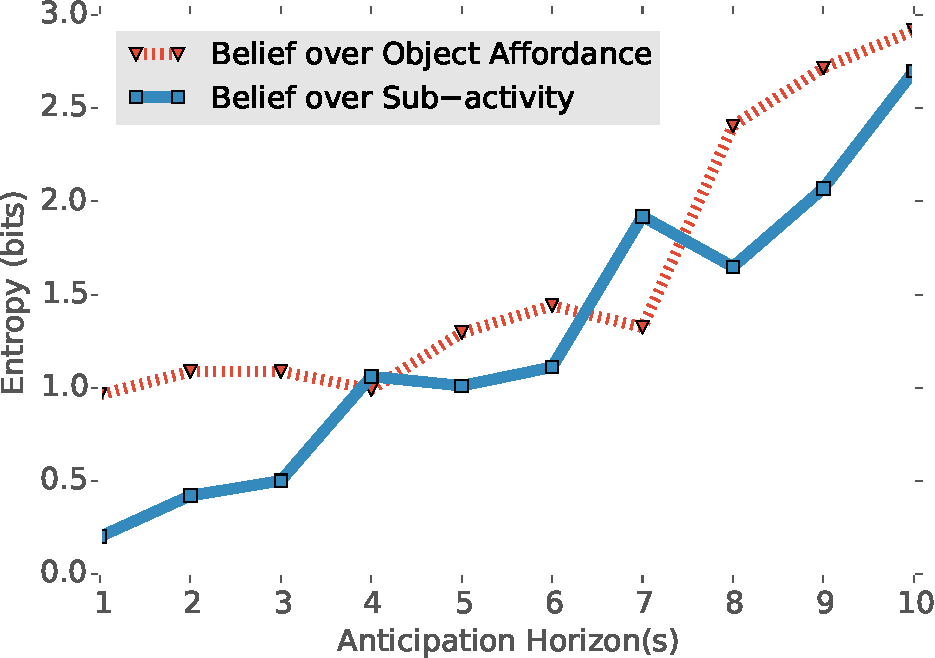
\includegraphics[width=\textwidth]{entTwo}
\caption{Entropy of the belief vs. time \emph{(uniform dist. has $\approx 3.32$ bit entropy)}}
\label{entRop}
\end{center}
\end{figure}

We further computed the entropy of the belief rCRF computes and plotted its average in Figure~\ref{entRop}. The decrease rate of the accuracy is much smaller than the increase rate of the entropy. In summary, recursive modeling is necessary for an accurate belief estimation and rCRF computes flatter yet still informative beliefs with increasing horizon.

\noindent {\bf How to efficiently cover the output space?}
In order to see the effect of structural diversity on covering the output space, we compare the rCRF with a version of it in which we replace diverse sampling with the Gibbs sampler. As expected, Gibbs sampler only sampled the small region around the posterior and failed to cover the output space. Within all experiments, rCRF outperforms Gibbs sampler baseline. Another interesting observation is, as shown in Figure~\ref{antHor}\&\ref{objHor}, although Gibbs sampler based method performed slightly better than other baselines for short horizon activity anticipation, it performed much worse for object affordance. We believe this is because of the dimensionality. Activity space has dimension $10^{T}$ whereas the object affordance space has dimension $12^{T\cdot M}$ where $T$ is the length of the video and $M$ is the number of objects. Hence, diversity plays bigger role with increasing dimension. Moreover, \cite{hemaAnt} uses the domain knowledge by selectively sampling points around the hand, etc. and it performs better than both baselines with increasing horizon. We believe this result is due to the efficient coverage of the output space with heuristics.

\begin{figure}[t]
  \centering
  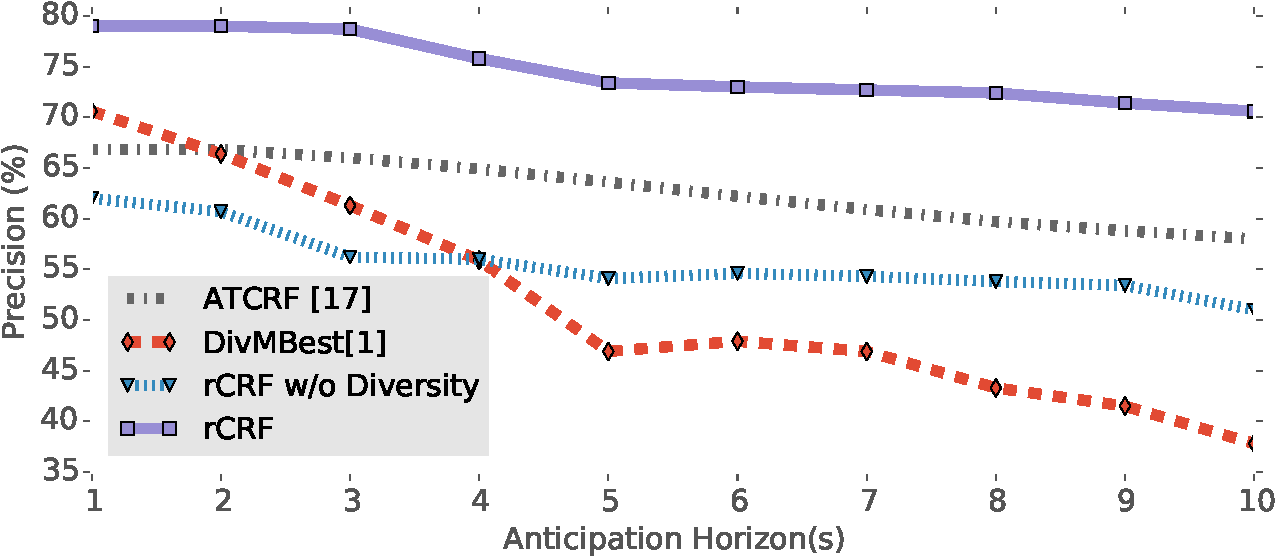
\includegraphics[width= \textwidth]{AntO}
\caption{Precision vs. anticipation horizon for object affordance.}
\label{antHor}
\end{figure}

\begin{figure}[h!]
  \centering
  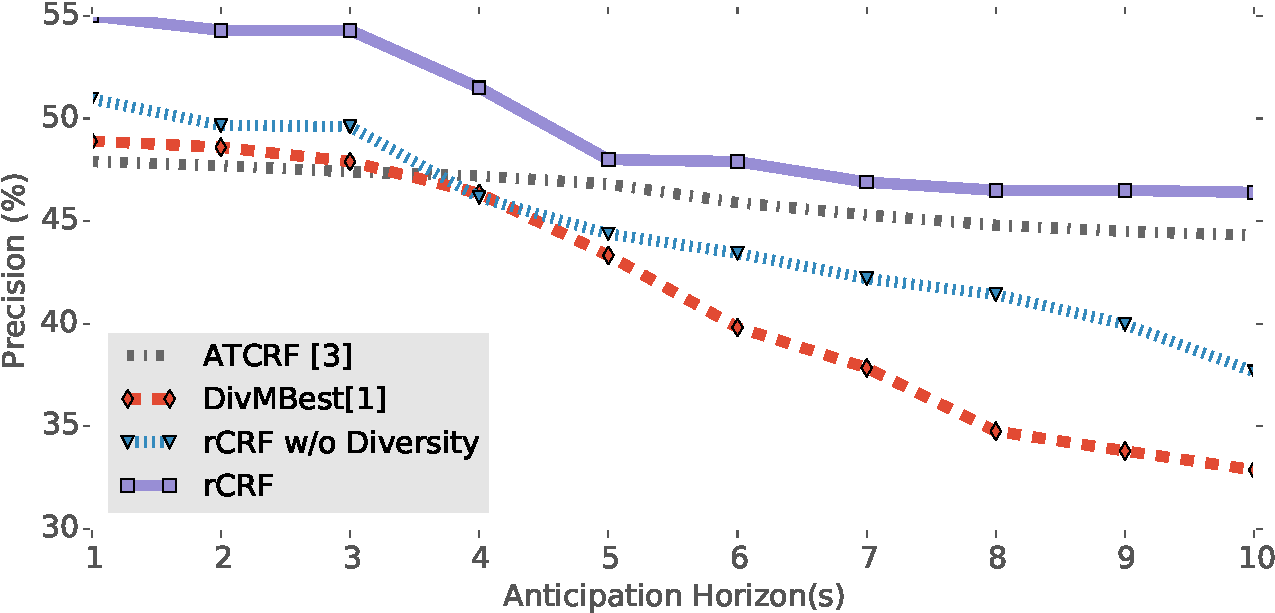
\includegraphics[width=\textwidth]{AntA}
\caption{Precision vs. anticipation horizon for subject activities.}
\label{objHor}
\end{figure}

\noindent {\bf Computationally-efficient inference:}
We evaluated the computational efficiency by computing the average computation time for anticipating 3 second in the future via rCRF and the fastest available anticipation algorithm (the ATCRF\cite{hemaAnt}). Within our experiments, we did not include any pre-processing or feature extraction computation (they are same for all algorithms). Our experiments suggest that the rCRF is faster than \cite{hemaAnt} as shown in Table~\ref{speed}. Hence, rCRF model outperforms the state-of-the-art anticipation algorithm in terms of speed in addition to the accuracy.
\begin{table}[h!]
  \centering
%  \vspace{-2mm}
\caption{Computation time for anticipating 3 seconds in the future excluding pre-processing (\emph{see supplementary material for details}).}
%\vspace{-2mm}
  \begin{tabular}{|cc|cc|}
    \hline
  ATCRF \cite{hemaAnt} \; \; & \; \; 34.1s  \; \;  \; & \; \; \;  rCRF \; \; & \; \;  1.41s \\ \hline
  \end{tabular}
  \vspace{-1mm}
  \label{speed}
\end{table}
%\vspace{-2mm}

\noindent {\bf Can rCRF generalize to RGB data?:}
Since there is no RGB activity dataset with object labels, it is hard to compare our algorithm in the RGB activity analysis setting. Removing the concept of the objet form the graph, makes it a chain-CRF and the inference and learning becomes straightforward. However, we still implement our rCRF over a linear-chain CRF for RGB activity analysis. We based our implementation on MPII cooking activity dataset \cite{mpi_cooking} and use the publicly distributed features from the authors webpage. The shared features are HOG, HOF, dense trajetory features and  MBH \cite{dalal}.


%\begin{table}
\begin{table}
  \caption{Anticipation performance for the anticipating 3 seconds in the future in MPII Cooking Dataset\cite{mpi_cooking}.}
\begin{tabular}{l|ccc} \hline
& micro & macro & macro  \\
Method & prec(\%) & prec(\%) & recall(\%) \\ \hline
Chance & $1.5${\scriptsize $\pm 0.6$} & $1.5${\scriptsize $\pm 0.6$}  & $1.5${\scriptsize $\pm 0.6$}  \\
ATCRF \cite{hemaAnt} & $33.4${\scriptsize $\pm 3.3$} & $52.1${\scriptsize $\pm 4.6$}  & $12.1${\scriptsize $\pm 1.4$}  \\
DivMBest\cite{divmbest} & $34.4${\scriptsize $\pm 2.8$} & $55.3${\scriptsize $\pm 5.0$}  & $14.3${\scriptsize $\pm 1.2$}  \\
rCRF & $\mathbf{37.4}${\scriptsize $\mathbf{\pm 2.9}$} & $\mathbf{63.2}${\scriptsize $\mathbf{\pm 5.5}$}  & $\mathbf{26.1}${\scriptsize $\mathbf{\pm 2.6}$}  \\
\hline
\end{tabular}
\label{Tantmpi}
\end{table}

As shown in the Table~\ref{Tantmpi}, our method outperforms all baselines and competing algorithms. We did not include Gibbs sampling here since the dimension of the activity space is rather low and the experiment over diversity is not informative. We believe this result is due to the accurate handling of temporal information in rCRF and it shows that it generalizes to other modalities.
